\section{Referencial Teórico}
\addcontentsline{toc}{section}{Referencial Teórico}

\subsection{L-System}
Originalmente como uma proposta matemática para a geração e simulação de plantas, foi apresentada por Lindenmayer\cite{Prusinkiewicz} para a área de botânica. Trata-se de um sistema que permite a construção de objetos complexos através de uma estrutura simples, tudo seguindo regras de substituição determinadas anteriormente, isso torna uma formula de reescrita de palavras, aplicando de forma paralela e simultânea a substituição de todos os elementos da palavra dada. 

O seu sistema mais simples é denominado de DOL-sistema, onde se possui um alfabeto, axioma e o conjunto de regras de tratamento. Essa estrutura é uma gramatica determinística e livre de contextos onde todas as regras são aplicadas simultaneamente no axioma. Se for considerado um	a palavra com duas letras 'a' e 'b', cada uma delas teria uma regra de reescrita. Considerando 'A' como o estado inicial da estrutura, onde possui as regras de produção como 'A' -> 'AB' e 'B' -> 'A', irá ter em sua execução durante suas gerações como na figura \ref{LSystemGenerationExemple} .

\begin{figure}[!h]
	\centering
	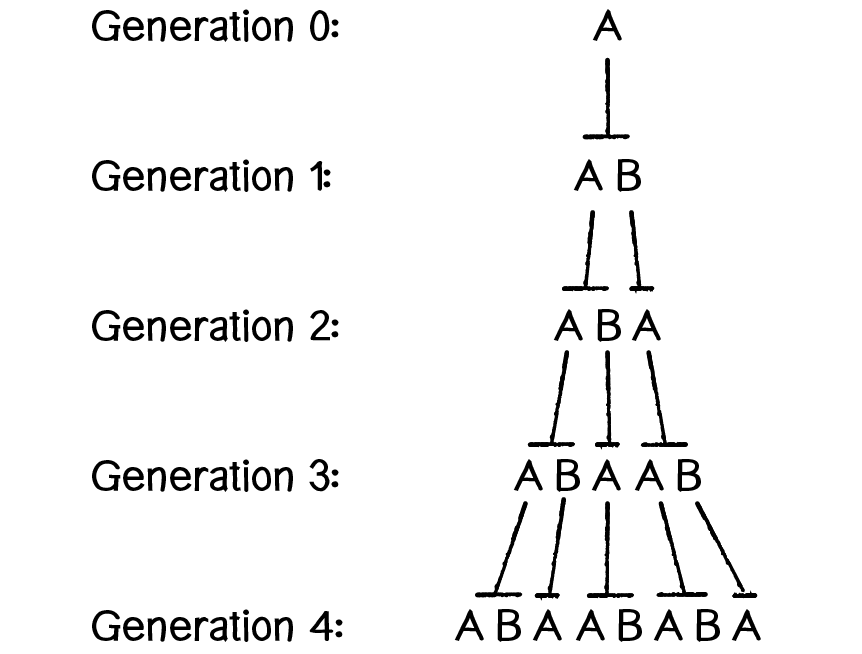
\includegraphics[width=0.5\textwidth]{LSystemExample}
	\caption{Gerações da estrutura seguindo a aplicação do L-System. Fonte: \cite{natureCode}}
	\label{LSystemGenerationExemple}
\end{figure}

Pode-se criar diversas estruturas usando essa técnica, na figura \ref{LSystemStructureExample3D} tem uma variação da curva de Hilbert 3D.

\begin{figure}[!h]
	\centering
	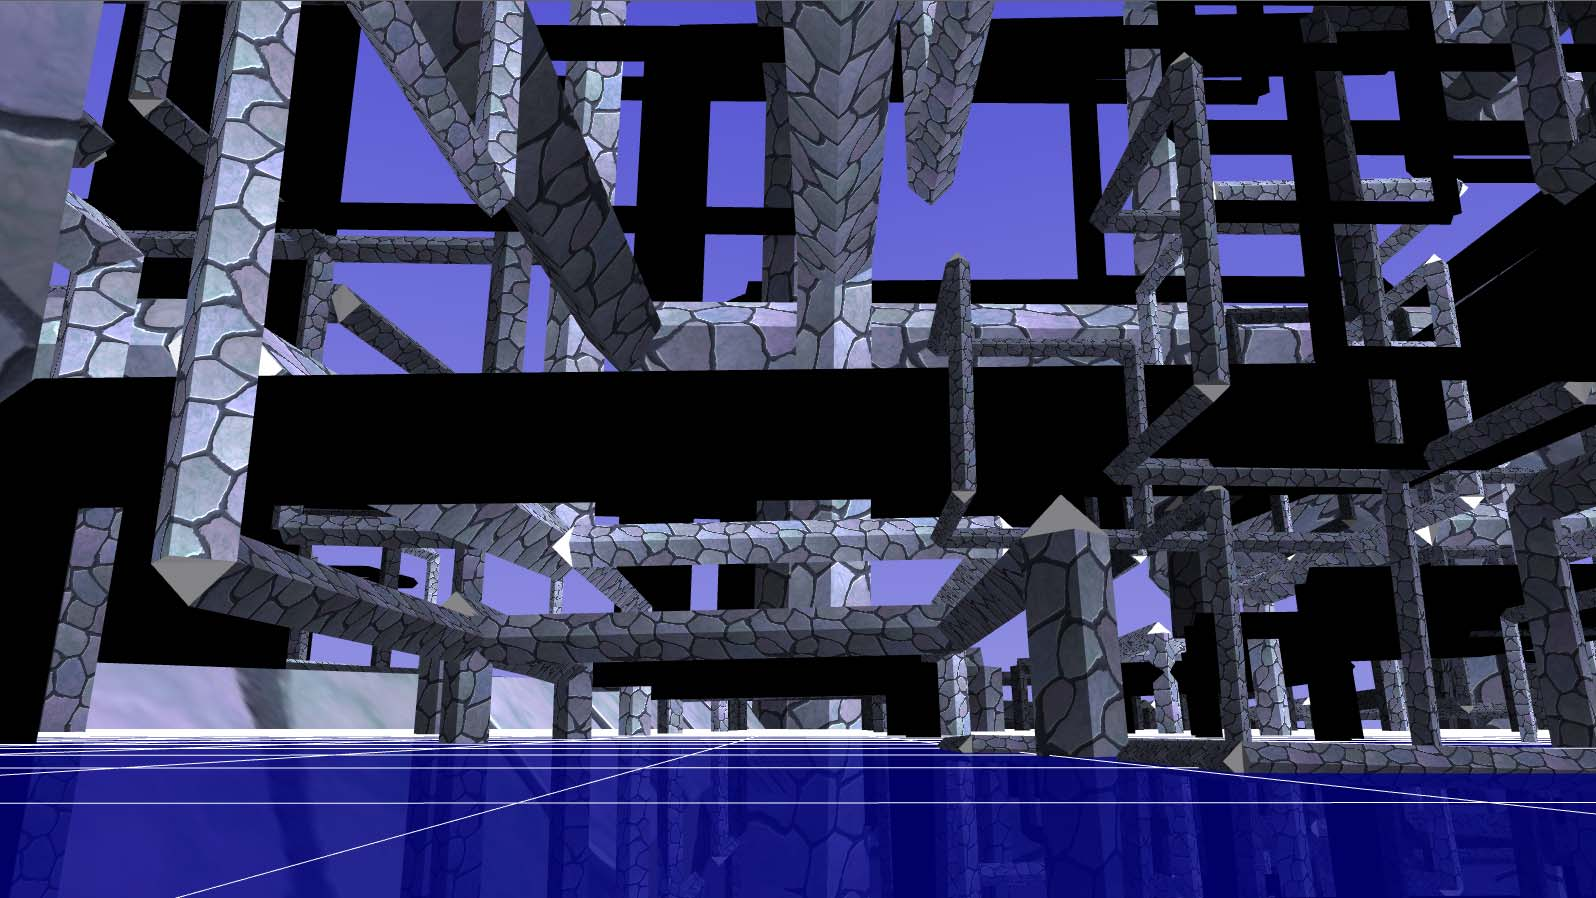
\includegraphics[width=0.3\textheight]{LSystemExample_3D}
	\caption{Exemplo de estrutura criada com L-System. Fonte: \cite{fridenfalk2015application}}
	\label{LSystemStructureExample3D}
\end{figure}

\subsection{Turtle Graphics} 
Turtle Graphics\cite{Abelson} é o método da interpretação gráfica da estrutura criada pelo L-System, sua ideia básica é a suposição de uma tartaruga posicionada no plano cartesiano, a tartaruga é definida por uma tupla <(x,y), $\alpha$ >, onde as coordenadas (x,y) indicam a posição da tartaruga e $\alpha$ o seu angulo.
Dando assim um passo d e um incremento de angulo fixo $\delta$, a tartaruga ira poder responder a comandos simples como apresentados na tabela \ref{turtleExempleRules}

\begin{table}[!h]
	\centering
	\begin{tabular}{|l|l|}
		\hline
		F & \begin{tabular}[c]{@{}l@{}}Mova um passo a frente de distancia d \\ desenhando uma linha.\end{tabular} \\ \hline
		f & \begin{tabular}[c]{@{}l@{}}Mova um passo a frente sem \\ desenhar uma linha.\end{tabular}              \\ \hline
		+ & Gira a esquerda por um ângulo.                                                                          \\ \hline
		- & Gira a direita por um ângulo.                                                                       \\ \hline
	\end{tabular}
	\caption{Exemplos de símbolos e comandos}
	\label{turtleExempleRules}
\end{table}

\subsection{Geração Procedural}
Em \cite{togelius2013procedural} refere a geração procedural de conteúdo á algoritmos capazes de gerar conteúdos para jogos, esses que podem ser dungeons, musicas, texturas, narrativas, entre outros.

Graças a esses algoritmos diminui os custos e tempo de produção desses elementos, dando a possibilidade aos desenvolvedores de se concentrarem em outros aspectos do jogo. Outra vantagem é que essas técnicas são capazes de aumentarem as variedades dos elementos no jogo, aumentando as experiencias do jogador durante suas jogatinas.

\subsection{Unity 3D}
Um motor de jogos proprietário desenvolvido pela Unity Technologies, permite a implementação dos jogos desenvolvidos nela em diversas plataformas como computadores (Windows, Linux, Mac), dispositivos moveis(Android,IOS), WebGL. Apesar da Unity ser um motor em C++, sua API(Application Programming Interface) para os desenvolvedores é em C\# junto com a plataforma Mono, dando a capacidade de rodar em diversos dispositivos. Graças a essas funcionalidades e sua facilidade de desenvolvimento ela tornou-se um dos principais motores entre os desenvolvedores indies. Ela possui um serviço chamado Unity Asset Store, aonde os desenvolvedores buscam assets para contribuir em seus projetos, desde sprites de personagens e modelos 3D até sistemas de jogos completos.